\subsubsection{UC12 - Effettua una prenotazione}
 \begin{figure}[h]
	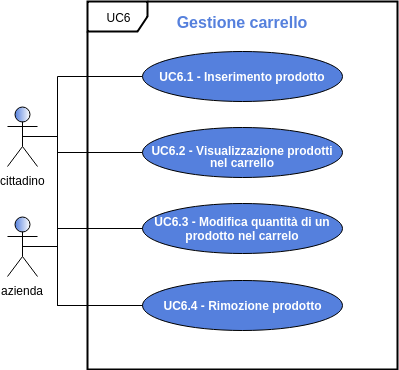
\includegraphics[width=6cm]{res/images/UC6GestioneCarrello.png}
	\centering
	\caption{UC11 - Effettua prenotazione}
\end{figure}
\begin{itemize}
	\item \textbf{Attori Primari}: utente autenticato;
	\item \textbf{Descrizione}: agli utenti autenticati è resa disponibile una maschera che presenta la lista di tutte le sue prenotazioni, dalla quale l'utente può scegliere di effettuare operazioni di gestione su ognuna di esse;
	Per ogni prenotazione presente nella lista saranno visualizzati dei dettagli riassuntivi, che sono:
	\begin{itemize}
		\item \textit{da completare in seguito}.
	\end{itemize}
	\item \textbf{Scenario principale}: l'utente effettua operazioni di gestione di una prenotazione. Esse comprendono:
	\begin{enumerate}[label=\alph*.]
		\item la visualizzazione dei dettagli di una prenotazione [UC11.1];
		\item la modifica di una prenotazione [UC11.2];
		\item la cancellazione di una prenotazione [UC11.3].
	\end{enumerate}
	\item \textbf{Precondizione}: il sistema riconosce l'utente proprietario o usufruente e rende disponibile il servizio di gestione delle prenotazioni;
	\item \textbf{Post-condizione}: l'utente riconosciuto può procedere con le operazioni di gestione rese disponibili.
\end{itemize} 
